% Formelsammlung für Elektrotechnik ZHAW IT HS2020
%
% Dokumenteinstellungen
% ======================================================================

% Dokumentklasse (Schriftgröße 8, DIN A4, Artikel)
\documentclass[8pt,a4paper]{scrartcl}

% Zusätzliche Pakete laden
\usepackage[utf8]{inputenc}        % Zeichenkodierung: UTF-8 (für Umlaute)
\usepackage[german]{babel}        % Deutsche Sprache
\usepackage{multicol}            % Spaltenpaket
\usepackage{amsmath}            % erlaubt mathematische Formeln
\usepackage{amssymb}            % Verschiedene Symbole
\usepackage{esint}                % erweiterte Integralsymbole
\usepackage{booktabs}            % bessere Tabellenlinien
\usepackage{graphicx}            % Zum Bilder einfügen benötigt
\usepackage{color}                % Farbiger Text möglich
\usepackage{pbox}                % Intelligent parbox: \pbox{maximum width}{blabalbalb \\ blabal}
%\usepackage{undertilde}            % Für Welle unterhlab von Matrixbuchstaben benötigt
\usepackage{accents}            % Für eigene Ableitungspunkte benötigt
\usepackage{scrtime}
\usepackage{supertabular}        % Für lange Tabellen mit Umbruch
\usepackage{pdfpages}
\usepackage{trfsigns}            % Laplace und Fourier
\usepackage{array}


% Seitenlayout und Ränder:
\usepackage{geometry}
\geometry{a4paper,landscape, left=6mm,right=6mm, top=-1mm, bottom=5mm,includeheadfoot}
\setlength{\parindent}{0mm}


% Dokumentbeschreibung
\title{Formelsammlung Elektrotechnik ZHAW IT HS2020}
\author{Andreas Sprecher}


% Kopf- und Fußzeile
% ======================================================================
\usepackage{fancyhdr}
\pagestyle{fancy}
\fancyhf{}
   \fancyfoot[C]{\textbf{Elektrotechnik}, Seite \thepage}
   \renewcommand{\headrulewidth}{0.0pt} %obere Linie ausblenden
   \renewcommand{\footrulewidth}{0.1pt} %obere Linie ausblenden

   \fancyfoot[R]{Stand: \todayV}
   \fancyfoot[L]{Andreas Sprecher}
% ----------------------------------------------------------------------

% Ausgegraut zum Abschreiben:
%\definecolor{grey}{rgb}{0.6,0.6,0.6}
%\color{grey}

% Eigene Befehle und Befehlsüberschreibungen
% ======================================================================

% Schriftart SANS für bessere Lesbarkeit bei kleiner Schrift
\renewcommand{\familydefault}{\sfdefault}
% Array- und Tabellenabstände vergrößern
\renewcommand{\arraystretch}{1.2}

% Befehle sichern
\let\oldvec = \vec
\let\olddot = \dot

% Eigene Befehle
\newcommand{\todayV}{\the\day.\the\month.\the\year}                          %%D.M.YYYY

\newcommand{\iset}[2]{\ensuremath{\bigl\{ \bigl. #1 \, \bigr| \, #2 \bigr\}}}                   % intensional set
\newcommand{\eset}[1]{\ensuremath{\bigl\{#1\bigr\}}}                                            % extensional set
%\newcommand{\enbrace}[1]{\ensuremath{\bigl\(#1\bigr\)}}                                        % extensional set
\newcommand{\enbrace}[1]{\ensuremath{\left(#1\right)}}
\newcommand{\norm}[1]{\ensuremath{\|#1\|}}                                                      % Norm
\newcommand{\mat}[1]{\ensuremath{\begin{bmatrix} #1 \end{bmatrix}}}                             % Matrix
\newcommand{\ma}[1]{\ensuremath{\boldsymbol {#1}}}                                              % Matrixsymbol
\newcommand{\vect}[1]{\ensuremath{\begin{pmatrix} #1 \end{pmatrix}}}                            % Vektor
\newcommand{\mvect}[1]{\ensuremath{\left. \begin{matrix} #1 \end{matrix}  \right]}}             % Matrixvektornotation
\newcommand{\gk}[1]{\ensuremath{\left\lfloor#1\right\rfloor}}                                   % Gaußklammer
\newcommand{\sprod}[2]{\ensuremath{\left\langle #1, #2 \right\rangle }}                         % Skalarprodukt
\newcommand{\abs}[1]{\ensuremath{\left\vert#1\right\vert}}                                      % Betrag
\newcommand{\bdot}{\ensuremath{\boldsymbol \cdot}}                                              % Dicker Punkt für Skalarprodukt
\newcommand{\svdots}{\ensuremath{\olddot :}}                                                    % small vertical dots
\newcommand{\mustbe}{\stackrel{!}{=}}

\newcommand{\inn}{\operatorname{int}}


% Überschreibungen
\renewcommand{\vec}[1]{\ensuremath{\boldsymbol {#1}}}                                           % Vektor fett und unterstrichen
\renewcommand{\emph}[1]{\textbf{#1}}                                                            % Hervorhebungen fett
\renewcommand*{\dot}[1]{\accentset{\mbox{\textrm{\large\bfseries .}} }{#1}}                     % Dicker Ableitungspunkt
\renewcommand*{\ddot}[1]{\accentset{\mbox{\textrm{\large\bfseries .\hspace{-0.25ex}.}}}{#1}}    % Dicker Doppelableitungspunkt

% Abkürzungen
\newcommand{\ul}[1]{\ensuremath{\underline{#1}}}                               % Untersteichen
\newcommand{\ol}[1]{\ensuremath{\overline{#1}}}                                % Überstreichen
\newcommand{\Ra}[0]{\ensuremath{\Rightarrow}}                                  % Rightarrow
\newcommand{\ra}[0]{\ensuremath{\rightarrow}}                                  % Rightarrow
\newcommand{\bs}[1]{\ensuremath{\boldsymbol{#1}}}                              % Fett und kursiv im mathmode
\newcommand{\diff}{\ensuremath{\;\mathrm d}}                                   % differentielles delta
\newcommand{\grad}{\ensuremath{\mathrm{grad}\ }}                               % Gradient
\renewcommand{\div}{\ensuremath{\mathrm{div}\ }}                               % Divergenz
\newcommand{\rot}{\ensuremath{\mathrm{rot}\ }}                                 % Rotation
\newcommand{\Sp}{\ensuremath{\mathrm{Sp}\ }}                                   % Spur
\renewcommand{\i}{\ensuremath{\mathrm{i}}}                                     % Imaginäre Einheit

% Für Mengen
\newcommand{\N}{\ensuremath{\mathbb N}}
\newcommand{\R}{\ensuremath{\mathbb R}}
\newcommand{\C}{\ensuremath{\mathbb C}}


%Custom functions
\DeclareMathOperator{\arccot}{arccot}


% Dokumentbeginn
% ======================================================================
\begin{document}


% Aufteilung in Spalten
\begin{multicols*}{3}
\setlength{\columnseprule}{0.4pt}
    \parbox{4cm}{
        \includegraphics[height=2cm]{./img/Logo.jpeg}
    }
    \parbox{4cm}{
        \emph{\Large{Elektrotechnik}}
    }
    \vspace{-2mm} 

    \section{Grundlagen}
		\subsection{Zentrale Aufgaben der Physik}    
    			\begin{itemize}\itemsep0pt				
				\item Angabe von Datenstrukturen, welche Eigenschaften der Welt beschreiben.
				\item Angabe von Gesetzmässigkeiten, welche die Grössen von Eigenschaften miteinander in Beziehung setzen
				\item Angabe von Gesetzmässigkeiten, welche beschreiben, wie sich diese Eigenschaften als Funktion der Zeit verändern.
			\end{itemize}
    
    		\subsection{Fundamentalkräfte}
			\begin{itemize}\itemsep0pt				
				\item Gravitation
				\begin{itemize}\itemsep0pt				
					\item Zwischen zwei Massen wirkt eine Anziehungskraft
					\item Kraft wirkt umgekehrt proportional zum Abstand der Masse
					\item Kraft wirkt proportional zum Produkt der Masse
					\item Ist nicht abschirmbar
				\end{itemize}
				\item Elektromagnetismus				
				\begin{itemize}\itemsep0pt				
					\item Grundursache is die elektrische Ladung
					\item Dualismus, Zwei Arten: positive und negative Ladung
					\item Gleiche Ladung stosst sich ab, unterschiedliche Ladung zieht sich an
					\item In allen physikalischen Prozessen bleibt die Ladung erhalten
					\item Einheit der Ladung: Coulomb[c] Elektron Ladung e = $1.602*10^{-19}C$
				\end{itemize}
				\item Starke Kernkraft		
				\item Schwache Kernkraft
			\end{itemize}
			
			\subsection{Kräfte}
				\begin{itemize}\itemsep0pt					
					\item Eine Kraft verändert die Geschwindigkeit eines Objektes, d.h. das Objekt wird beschleunigt (oder gebremst). 
				\end{itemize}
				\subsubsection{Beschleunigung}
					\begin{itemize}\itemsep0pt				
						\item $F=ma$
					\end{itemize}
				\subsubsection{Schwerkraft}
					\begin{itemize}\itemsep0pt				
						\item $F=\gamma\dfrac{M_{1}M_{2}}{r^{2}}, \gamma = 6.67*10^{-11}\dfrac{Nm^{2}}{kg^{2}}$
						\item Erde: $F =mg, g = \gamma\dfrac{M_{Erde}}{r_{Erde}^{2}}=9.81\dfrac{m}{s^{2}}$
					\end{itemize}
				\subsubsection{Coulombkraft}
					\begin{itemize}\itemsep0pt				
						\item $\overrightarrow{F_{12}}=\dfrac{Q_{1}Q_{2}}{4\pi\varepsilon_{0}r^{2}}, \varepsilon_{0}=8.859*10^{-12}\dfrac{C^{2}}{Jm}$
					\end{itemize}
				\subsubsection{Federkraft}
					\begin{itemize}\itemsep0pt				
						\item $F = -k(x-x_{Ruhe})$
					\end{itemize}
			
		\subsection{Energie}
			\begin{itemize}\itemsep0pt				
				\item $E_{pot}=mgh$
				\item $E_{kin}=m\dfrac{v^{2}}{2}$
				\item $E_{spring}=k\dfrac{(x-L)^{2}}{2}$, $(x-L)$: Auslenkung
				\item $E_{pot. Ladung}=qU$
				\item Arbeit: $\Delta E_{mech}=Fs$			
			\end{itemize}
			\subsubsection{Einheiten}		
			\begin{itemize}\itemsep0pt		
				\item $1 cal = 4.1868 J$		
				\item $[J]=[Nm]$
				\item $[N]=[\dfrac{Km}{s^{2}}]$
			\end{itemize}

		\subsubsection{Energieerhaltung}			
			\begin{itemize}\itemsep0pt		
				\item In einem System und der Umgebung bleibt die \textbf{Gesamtmenge} der Energie erhalten			
				\item Veränderungen geschehen durch physikalische Kräfte
				\item Diese physikalischen Kräfte können nicht beliebig aussehen. Ihre Form ist z.B. durch die Forderung, dass die physikalischen Gesetze sich im Laufe der Zeit nicht ändern, etwas eingeschränkt
				\item Diese Einschränkung führt dazu, dass einem physikalischen System eine Zahl zugeordnet werden kann, deren Grösse durch die Einwirkung der Kräfte nicht geändert werden kann
				\item Die Erhaltung der Energie ist nicht eine Folge einer Energiesubstanz
				\item Die Gesetze der Physik sind so gestaltet, dass sie die Gesamtmenge der Energie nicht verändern können
				
			\end{itemize}

		\subsection{Strecke, Geschwindigkeit, Beschleunigung}
			\begin{itemize}\itemsep0pt				
				\item $v=\int a \delta t$
				\item $s=\int v \delta t$
			\end{itemize}			
			
	\section{Veränderungsraten Leistung Strom}
		\subsection{Veränderungsraten}
			\begin{itemize}\itemsep0pt			
				\item Das zukünftige Verhalten eines Systems und seiner Umwelt ist vollständig definiert durch seinen momentanen Zustand und dem momentanen Zustand der Umwelt. Zusätzliche Information, z.B. wie diese Zustände erreicht wurden, sind nicht nötig.
				
			\end{itemize}
		\subsection{Potential }
			\begin{itemize}\itemsep0pt			
				\item $\varphi (A)=\dfrac{x}{y}$
				\item x = pot.E Substanz S der Menge M an Ort A
				\item y = Menge X Energietraeger
			\end{itemize}
			
		\subsection{Strom $I$}
			\begin{itemize}\itemsep0pt				
				\item $I [A] [\dfrac{C}{s}]$
				\item Richtung in die sich die positive Ladung bewegt $I>0$
				\item Anzahl positiver Ladung die den Querschnitt pro Sekunde durchquert
			\end{itemize}
			
		\subsection{Spannung $U$}
			\begin{itemize}\itemsep0pt				
				\item $U [V] [\dfrac{W}{A}]$
				\item $U=U(\overrightarrow{r_{A}},\overrightarrow{r_{B}})=\varphi(\overrightarrow{r_{A}})-\varphi(\overrightarrow{r_{B}})$
				\item Spannungsquellen erzeugt $\overrightarrow{E}$-Feld in Drähten
				\item Ladung verliert $\Delta E_{pot}$ und gewinnt $\Delta E_{kin}$
				\item Kinetische Energie kann Verbraucht werden
				\item Spannung ist die Energie die frei wird, wenn die Ladung von A nach B bewegt wird.
				\item $\varphi(\overrightarrow{r_{A}})>\varphi(\overrightarrow{r_{B}})$ Energie steht zur verfügung
				\item $\varphi(\overrightarrow{r_{A}})<\varphi(\overrightarrow{r_{B}})$ Energie wird benötigt
			\end{itemize}
			
		\subsection{Leistung $P$}
			\begin{itemize}\itemsep0pt
				\item $P: [\text{W}] = [\dfrac{J}{s}]$
				\item Energieänderung pro Zeitintervall
				\item Leistung kann aufgenommen oder abgegeben werden
				\item $P_{el}=\dfrac{\Delta E}{\Delta t} = \dfrac{I \Delta t U}{\Delta t} = UI$
				\item  $P_{\text{Hydraulik}}=p_{\text{diff}}I_{\text{V}}$
				\item  $P_{\text{Gravitation}}=g h_{\text{diff}}I_{\text{m}}$
				\item $P_{\text{rad}} = \sigma AT^{4}$, $\sigma = 5.67\cdot 10^{-8} [\dfrac{W}{m^{2}K^{4}}]$
				\item Wirkungsgrad $\eta = \dfrac{P_{\text{desired}}}{P_{\text{driving}}} \leq 1$
			\end{itemize}
			
		\subsection{Schaltung}
			\begin{itemize}\itemsep0pt
				\item Physikalische Perspektive
				\begin{itemize}\itemsep0pt
					\item Schaltungen bestehen aus miteinander verbundenen physikalischen Elementen, welche, angeregt durch Spannungen und Ströme, ein bestimmtes dynamisches Verhalten zeigen.
					\item Die physikalische Perspektive offeriert noch keine Semantik, zeigt aber, wie ein System gebaut werden kann.
				\end{itemize}					
			
				\item Funktionale Perspektive
				\begin{itemize}\itemsep0pt
					\item Schaltungen sind Signalwandler
					\item Logische Schaltungen: Input ist eine Bitsequenz, welche in eine Outputsequenz verwandelt wird.
					\item Analoge Schaltung: Ein dynamisches Signal wird in ein Outputsignal transformiert.
				\end{itemize}						
			\end{itemize}		
			\subsubsection{Analoge Schaltung}
				\begin{multicols*}{2}		
					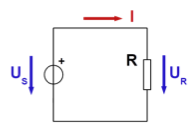
\includegraphics[height=3.3cm]{img/schaltung.png}
					\begin{itemize}\itemsep0pt				
						\item $R[\Omega]$
						\item $U_{R}=RI$
						\item $P=IU_{R}=\dfrac{U_{R}^{2}}{R}=RI^{2}$
					\end{itemize}
				\end{multicols*}
				\begin{itemize}\itemsep0pt
					\item Eine \textbf{Masche} oder Schlaufe ist ein Weg durch Drähte und Bauelemente, welcher zu seinem Ausgangspunkt zurückführt
					\item Die Spannung wird in Richtung Spannungsgefälle positiv gezählt
					\item Bei einem \textbf{Knoten} kommen mindestens drei Drähte zusammen.
					\item Durch die Ladungserhaltung muss die Summe der einfliessenden minus der Summe der wegfliessenden Ströme null ergeben.
					\item Kabelwiderstand $R = \rho\dfrac{L}{A}$							\end{itemize}			
				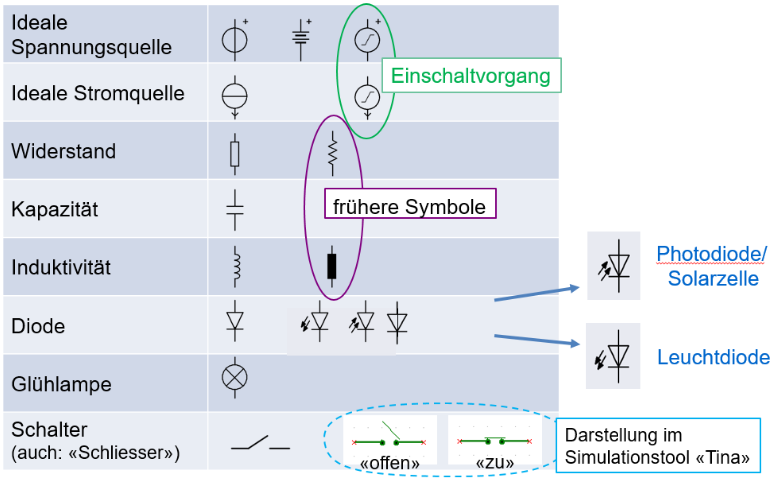
\includegraphics[height=5.5cm]{img/schaltung2.png}	
				\subsubsection{Serieschaltung}	
					\begin{itemize}\itemsep0pt
						\item Serieschaltung $R = R_{1} + R_{2}$
						\item Serieschaltung $I = \dfrac{U_{0}}{R_{1} + R_{2}}$
					\end{itemize}
				\subsubsection{Parallelschaltung}	
					\begin{itemize}\itemsep0pt
						\item Parallelschaltung $R=\dfrac{R_{1} \cdot R_{2}}{R_{1} + R_{2}}$
						\item Parallelschaltung $I_{0}=U_{0}(\dfrac{1}{R_{1}} + \dfrac{1}{R_{2}})$
					\end{itemize}
					
				\subsubsection{Mehrere Quellen}	
					\begin{itemize}\itemsep0pt
						\item Superpositionsprinzip: Jede Quelle wird einzeln analysiert und anschliessend wird addiert
						\item Analyse: Spannungsquellen werden durch einen Kurzschluss ersetzt, Stromquellen durch eine offene Verbindung
						\item Wenn Dioden vorkommen, ist die Schaltung nicht mehr linear, das Superkompositionsprinzip gilt nicht mehr
					\end{itemize}
			
			
		\subsection{Batterie}
			\begin{multicols*}{2}
				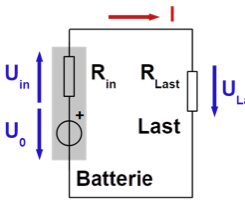
\includegraphics[height=3.3cm]{img/batterie.png} \\
				\begin{itemize}\itemsep0pt
					\item Ideale Bat: $U_{0}=const.$				
					\item $U_{0}-U_{in}-U_{last} =0$
					\item $U_{0}-IR_{in}-IR_{last} =0$
					\item $I=\dfrac{U_{0}}{R_{in}+R_{last}}$
					\item $P=R_{la.}(\dfrac{U_{0}}{R_{in}+R_{la.}})^{2}$
				\end{itemize}
			\end{multicols*}
			\begin{itemize}\itemsep0pt
				\item Wenn der Laswiederstand kleiner als der Innenwiderstand ist, wird die Leistung bei kleinerem Lastwiederstand nicht grösser
				\item Wenn ein Verbraucher mit einer Batterie betrieben wird, muss aufgepasst werden, dass die Leistung nicht am Innenwiderstand der Batterie verbraucht wird
				\item Bei einer Gleichspannungsquelle mit variabler Spannung, z.B. einer Solarzelle, muss der Lastwiderstand dynamisch anpasst werden (Bei Solarpaneln ist der Lastwiderstand der gleich wie beim Speicher)	
				
			\end{itemize}
			
		\subsection{Kondensator}
			\begin{multicols*}{2}
				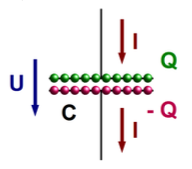
\includegraphics[height=3.8cm]{img/kondensator1.png} 
				
				\begin{itemize}\itemsep0pt
					\item Kondensatoren können praktisch beliebig oft auf- und entladen werden
					\item Kondensatoren können als Energiespeicher verwendet werden (Bremsenergie)
					\item Kapazität C [Farad/F]
					\item $\dfrac{\delta Q} {\delta t} = I$
					\item $CU_{c}=Q$
				\end{itemize}
				
			 \end{multicols*}
			 
			 \begin{multicols*}{2}
				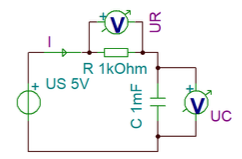
\includegraphics[height=3.1cm]{img/kondensator2.png} 
				
				\begin{itemize}\itemsep0pt
					\item $I = \dfrac{1}{R}(U_{s}-\dfrac{Q}{C})$
					\item $U_{s}=IR+\dfrac{Q}{C}$
				\end{itemize}
				
				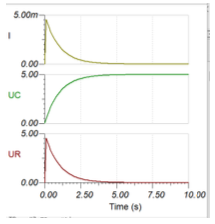
\includegraphics[height=4.4cm]{img/kondensator3.png} 

			 \end{multicols*}

		\subsection{Hochspannung}
			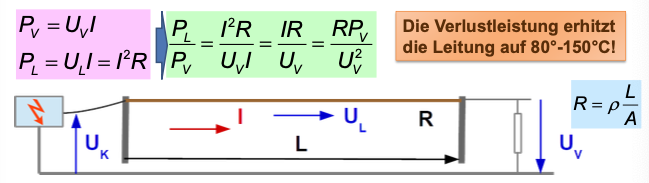
\includegraphics[height=2.5cm]{img/hochspannung1.png} 
			\begin{itemize}\itemsep0pt
				\item Je grösser $U_{V}$, desto kleiner der relative Leistungsverlust in der Leitung.
				\item Der Verlust beträgt wenige Prozent pro hunder Kilometer (Wechselspannung)
			\end{itemize}
			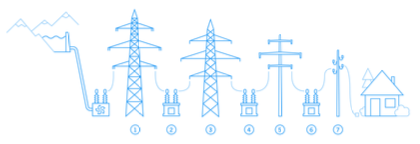
\includegraphics[height=2.2cm]{img/hochspannung2.png} 
			\begin{itemize}\itemsep0pt
				\item 1 Höchstspannung: 380 kV beziehungsweise 220 kV 
				\item 3 Hochspannungsebene: 36 kV bis 150 kV
				\item 5 Mittelspannungsebene: 1 kV bis 36 kV
				\item 7 Niederspannungsebene: $<$ 1 kV 
				\item 2,4,6 Transformatorenebenen 
			\end{itemize}
		\subsection{Gleich- und Wechselstrom}
			\begin{itemize}\itemsep0pt
				\item Historisch bedingt konnte früher nur Wechselstrom transformiert werden. 
				\item Wechselstrom relativ hohe Verlustleistung (Skineffekts, ..)
				\item Gleichstrom hat eine geringere Verlustleistung.
			\end{itemize}

		\section{Digitaltechnik}
			\subsection{Funktionseinheiten \& Signale}
				\begin{itemize}\itemsep0pt
					\item Eine \textbf{Funktionseinheit} empfangt n Inputsignale und liefert m Outputsignale
					\item Eine \textbf{Rückkopplung} ist beispielsweise wenn Outputsignal von FE1 Inputsignal von FE2 ist und ein Outputsignal von FE2 ein Inputsignal von FE1 ist.
					\item \textbf{Schaltnetze} enthalten mehrere Funktionseinheiten ohne Rückkopplungen.
					\item \textbf{Schaltwerk} enthalten Rückkopplungen und besitzen dadurch einen speichernden Charakter.
				\end{itemize}
			\subsection{Logik-Gatter}
				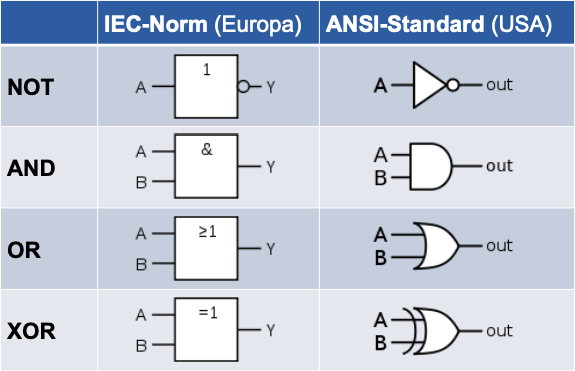
\includegraphics[height=5.8cm]{img/digitaleGrundbausteine.png} 
				\begin{itemize}\itemsep0pt
					\item Schalter die durch elektronische Signale betrieben werden sind \textbf{Transistoren}
					\item NOT: Einzelner Schalter
					\item AND: Zwei Schalter in serie
					\item OR: Zwei Schalter parallel
					\item XOR: Zwei Schalter in serie versetzt
				\end{itemize}
			
			\subsection{Flip-Flops}
			Ein Flip-Flop ist das fundamentale Speicherelement.
				\subsubsection{SR-Flip-Flop}
					\begin{itemize}\itemsep0pt
						\item Input S und R
						\item Funktioniert nur wenn S und R unterschiedlich oder beide Null sind (Beide Null speichert)
						\item Q = S
					\end{itemize}
					
				\subsubsection{D-Flip-Flop}
					\begin{itemize}\itemsep0pt
						\item S und R werden zu D zusammengefasst
						\item Wenn der Clockeingang von unten nach oben wechselt wird der Speicher gesetzt (flankengesteuert)
					\end{itemize}
					
				\subsubsection{JK-Flip-Flop}
					\begin{itemize}\itemsep0pt
						\item S wird mit J(Jump) und R mit K(Kill) ersetzt
						\item Es gibt einen Clockeingang (flankengesteuert)
						\item Wenn beide Eins sind, wechselt der Ausgang bei jeder aktiven Clockflanke
					\end{itemize}
					
				\subsection{KV-Diagramm}
					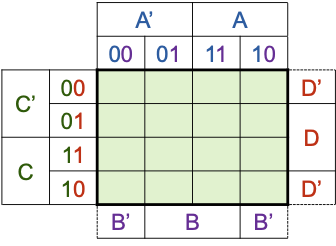
\includegraphics[height=6.5cm]{img/kv1.png} \\
					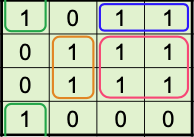
\includegraphics[height=3cm]{img/kv2.png} 
					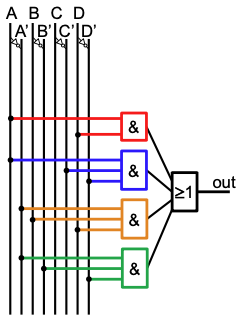
\includegraphics[height=7cm]{img/kv3.png} 
				
				\subsubsection{Glitches}
					\begin{itemize}\itemsep0pt
						\item Wenn beim Schaltungsentwurf jeder Signalpfad die selbe Anzahl Logikgatter durchläuft, können Gliches vermieden werden
						\item KV-Diagramme allein sind daher kein gutes Entwurfsmuster für glitchfreie Schaltungen
						\item Wird bei einem RLC-Schwingkreis die Induktivität erhöht, verkürzt sich die Periodendauer nicht
					\end{itemize}


		\section{Elektrische und Magnetische Felder}

			\subsection{Ladungen und Ströme}
				\begin{itemize}\itemsep0pt
					\item \textbf{Superpositionsprinzip}: Sind mehrere Ladungen vorhanden, werden die Kräfte zusammengezählen
					\item $\overrightarrow{F_{12}}$: Kraft auf Ladung $Q_{1}$, verursacht durch Ladung $Q_{2}$
					\item Einheitsvektor von $Q_{2}$ zu $Q_{1}$: $\overrightarrow{n}_{12} = \dfrac{\overrightarrow{r}_{12}}{|\overrightarrow{r}_{12}|}$
					\item Permittivität des Vakuums $ \varepsilon_{0}=8.859*10^{-12}\dfrac{C^{2}}{Jm}$
				\end{itemize}
			
			\subsection{Coulombgesetz}
				\begin{itemize}\itemsep0pt
					\item $\overrightarrow{F}_{12}=\dfrac{1}{4\pi\varepsilon_{0}}\dfrac{Q_{1}Q_{2}}{|\overrightarrow{r}_{12}|^{2}}\overrightarrow{n}_{12}$
				\end{itemize}
			
			\subsection{Elektrische Felder}
			
				\begin{itemize}\itemsep0pt
					\item $\overrightarrow{E}(\overrightarrow{r},t), [\dfrac{N}{C}]$
					\item Werden erzeugt durch Ladung oder zeitlich veränderliche magnetische Felder
					\item Bei mehreren Quellen gilt das Superpositionsprinzip
					\item Das elektrische Feld zeigt von positiven Ladungen zu negativen Ladungen hin
					\item Das elektrische Feld übt eine Kraft aus, die proportional zur Stärke des Feldes ist
					\item Im Inneren eines geladenen Metallstück ist das elektrische Feld null
				\end{itemize}
			
				Ladung $Q$ an Ort $\overrightarrow{r}_{Q}$ erzeug $\overrightarrow{E}$-Feld:		
				\begin{itemize}\itemsep0pt
					\item $\overrightarrow{E}(\overrightarrow{r}) = \dfrac{1}{4\pi\varepsilon_{0}} \dfrac{Q}{|\overrightarrow{r}-\overrightarrow{r}_{Q}|^{2}}  \dfrac{\overrightarrow{r}-\overrightarrow{r}_{Q}}{|\overrightarrow{r}-\overrightarrow{r}_{Q}|}$
					
				\end{itemize}
				Kraft auf Ladung q am Ort 
				$\overrightarrow{r}$:
				\begin{itemize}\itemsep0pt
					\item $\overrightarrow{F}=q\overrightarrow{E}(\overrightarrow{r},t)$
				\end{itemize}
			\subsubsection{Elektronvolt}
				\begin{itemize}\itemsep0pt
					\item $1 eV = W = F \cdot d =q\cdot E\cdot d=q \cdot U= 1.6\cdot10^{-19}J$
					\item Arbeit $W=\dfrac{m\cdot v^{2}}{2}$
				\end{itemize}
			\subsection{Magnetische Felder}
				\begin{itemize}\itemsep0pt
					\item $\overrightarrow{B}(\overrightarrow{r},t), [\dfrac{kg}{s\cdot C}]$
					\item Werden erzeugt durch Ströme oder zeitlich veränderliche elektrische Felder
					\item Bei mehreren Quellen gilt das Superpositionsprinzip
					\item Das Magnetfeld zeigt vom Nord- zum Südpol
				\end{itemize}
				
				\subsubsection{Lorentzkraft}				
				
					\textbf{Lorentzkraft} auf Ladung q mit Geschwindigkeit $\overrightarrow{\nu}$:
					\begin{itemize}\itemsep0pt
						\item $\overrightarrow{F}_{L}=q\overrightarrow{\upsilon} $x$ \overrightarrow{B}$
					\end{itemize}	
					
					\textbf{Rechte Hand Regel}
					\begin{itemize}\itemsep0pt
						\item Mittelfinger: Richtung der Lorentzkraft
						\item Zeigefinger: Richtung des Magnetfeldes (Nord-Süd)
						\item Daumen: Richtung der positiven Ladung
					\end{itemize}		
					
					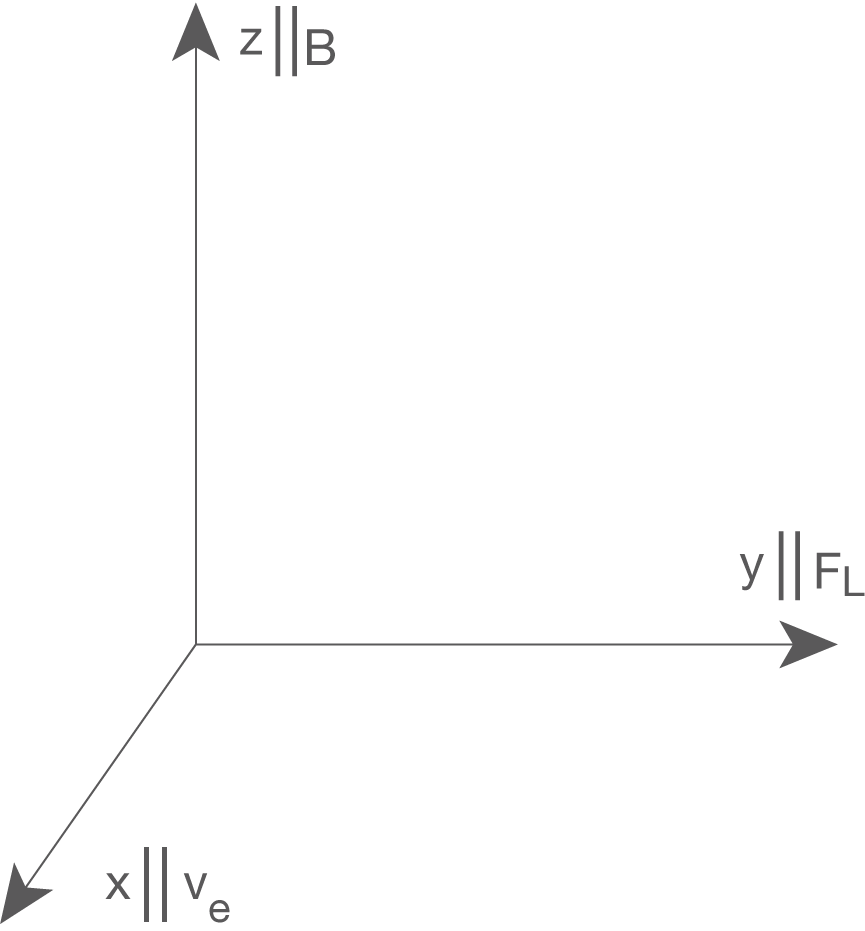
\includegraphics[height=4cm]{img/lorentzKoord.png} 
				
			\subsection{Generatoren/Elektromotoren}
				\begin{itemize}\itemsep0pt
					\item Steht ein stromdurchflossener Draht senkrecht zu einem Magnetfeld wirkt eine Kraft auf den Draht
				\end{itemize}	
			
					\subsubsection{Generatoren}
						\begin{itemize}\itemsep0pt
							\item Beim Generator werden die Leiterbahn im Magnetfeld bewegt
							\item Die Ladungsträger erhalten eine Geschwindigkeit senkrecht zur Leiterbahn
							\item Das Magnetfeld führt zu einer Kraft auf die Ladungsträger in Richtung der Leiterbahn
							\item Strom mit wechselnder Richtung (Wechselstrom) fliesst
						\end{itemize}
					\subsubsection{Elektromotoren}
						\begin{itemize}\itemsep0pt
							\item Beim Elektromoter werden die Leiterbahn im Magnetfeld durch die Lorentzkräfte bewegt
							\item Die stromdurchflossene Schlaufe führt zu einem Drehmoment
							\item Die Schlaufe dreht sich im Uhrzeigersinn
							\item Bei $\theta = 180$ wird die Stromrichtung geändert
						\end{itemize}		
						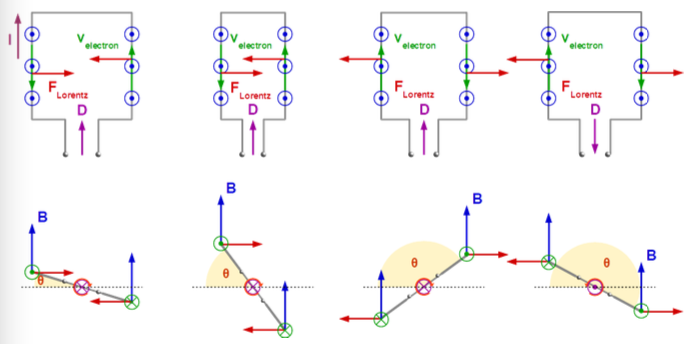
\includegraphics[height=4.6cm]{img/elemot.png} 
			\section{Maxwellgleichungen}
				\begin{itemize}\itemsep0pt
					\item Beschriebt unter anderem wie sich Licht als elektromagnetische Welle ausbreitet
				\end{itemize}				
			
			
				\subsection{Gauss’sches Gesetz (Elektrischer Fluss)}
					\begin{itemize}\itemsep0pt
						\item $\Phi_{\overrightarrow{E}}(\Sigma) = \int_{V}\dfrac{\rho}{\varepsilon_{0}}dV = \dfrac{Q}{\varepsilon_{0}}$
						\item Der Fluss des elektrischen Feldes $\overrightarrow{E}$ durch eine geschlossene Fläche $\Sigma$ ist gleich dem Volumenintegral über die Ladungsdichte $\rho / \varepsilon_{0}$ innerhalb von $\Sigma$, also gleich der von $\Sigma$ eingeschlossenen Ladung $Q$ geteilt durch $\varepsilon_{0}$
						\item $|\overrightarrow{E}| = \dfrac{Q}{4\pi\varepsilon_{0}r^{2}}$
						\item Das elektrische Feld zeigt von positiven Ladungen zu negativen Ladungen hin
					\end{itemize}		
				\subsection{Magnetischer Fluss}
					\begin{itemize}\itemsep0pt
						\item Es gibt keine magnetische Ladungen
						\item $\Phi_{\overrightarrow{B}}(\Sigma) =0$
						\item Der Fluss des magnetischen Feldes $\overrightarrow{B}$ durch eine geschlossene Fläche $\Sigma$ ist gleich 0
					\end{itemize}	
				\subsection{Faraday'sches Gesetz (Linienintegral des elektrischen Feldes)}
					\begin{itemize}\itemsep0pt
						\item $\int_{\gamma} \overrightarrow{E} \cdot d \overrightarrow{\gamma} = - \dfrac{d}{dt} \Phi_{\overrightarrow{B}}(\Omega)$
						\item Das Linienintegral des elektrischen Feldes $\overrightarrow{E}$ über einer Kurve $\gamma$ ist gleich der zeitlichen Änderung des negativen Flusses des magnetischen Feldes durch eine von $\gamma$ berandete Fläche $\Omega$
						\item Die Änderung des Flusses eines Magnetfeldes durch eine Schlaufe induziert in dieser eine Spannung U
						\item $U=-\dfrac{d}{dt}\Phi_{\overrightarrow{B}}$(Schlaufe)
						\item $\Phi_{\overrightarrow{B}}$(Schlaufe)=$\overrightarrow{A}\cdot \overrightarrow{B}$, $\overrightarrow{A}$ senkrecht Schlaufe Länge Fläche Schlaufe
						\item Spannung \textbf{Schlaufe}: $U_{ind}(t) = U_{0}sin(2\pi vt)$
						\item Amplitude: $U_{0} = \omega |\overrightarrow{A}||\overrightarrow{B}|$
						\item Frequenz: $v = \dfrac{\omega}{2\pi}$
						\item Kreisfrequenz: $\omega = 2\pi v$
					\end{itemize}	
				\subsection{Linienintegral des magnetischen Feldes}
					\begin{itemize}\itemsep0pt
						\item $\int_{\gamma} \overrightarrow{B} \cdot d \overrightarrow{\gamma} = \mu_{0}\Phi_{\overrightarrow{j}}(\Omega) + \mu_{0}\varepsilon_{0} \dfrac{d}{dt} \Phi_{\overrightarrow{E}}(\Omega)$
						\item Das Linienintegral des magnetischen Feldes $\overrightarrow{B}$ über einer Kurve $\gamma$ ist gleich der zeitlichen Änderung des Flusses des elektrischen Feldes (mal $\mu_{0}\varepsilon_{0}$) durch eine von $\gamma$ berandete Fläche $\Omega$ plus dem Fluss der Stromdichte durch $\Omega$ mal $\mu_{0}$
						\item Das Linienintegral des magnetischen Feldes $\overrightarrow{B}$ über einer Kurve $\gamma$ ist gleich der zeitlichen Änderung des Flusses des elektrischen Feldes (mal $\mu_{0}\varepsilon_{0}$) durch eine von $\gamma$ berandete Fläche $\Omega$ plus dem Fluss der Stromdichte durch $\Omega$ mal $\mu_{0}$
						\item $\mu_{0}= 1.26\cdot 10^{-6}[T\cdot m\cdot A^{-1}]$
						\item Magnetfeld um \textbf{langen geraden Leiter}: $B= \dfrac{\mu_{0}I}{2\pi r}$
						\item Magnetfeld in \textbf{Spuhle}: $B= \mu_{r} \mu_{0} \dfrac{N}{L}I$
					\end{itemize}	
					\textbf{Rechte Hand Regel}
					\begin{itemize}\itemsep0pt
						\item Daumen: Richtung der positiven Ladung
						\item Rest: Umlaufsinn des $\overrightarrow{B}$-Feldes um I
					\end{itemize}		
					
			\section{Frequenz und Kreisfrequenz}
				\begin{itemize}\itemsep0pt
					\item Frequenz : $f(t) = sin(2\pi vt)$
					\item Periode: $T = \dfrac{1}{v}$
					\item Kreisfrequenz: $\omega = 2\pi v$
				\end{itemize}	
				
				\subsection{Wechselstrom}
					\begin{itemize}\itemsep0pt
						\item Nennspannung : $U_{N} = \dfrac{U_{0}}{\sqrt{2}}$
						\item Spannung: $U(t) = U_{0}sin(2\pi vt + \phi_{0})$
						\item $U_{0}$: Amplitude
						\item $\phi_{0}$: Phasenkonstante
					\end{itemize}	
				\subsection{Transformatoren}
					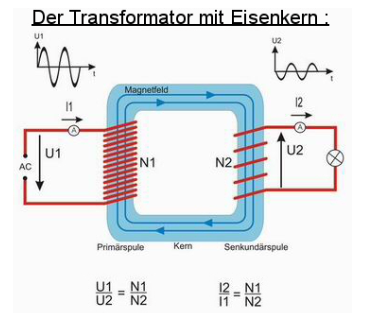
\includegraphics[height=7cm]{img/transformator.png} 
					
			\section{Wellen}
				\subsection{Wellengleichung}
				\begin{multicols*}{2}
					\begin{itemize}\itemsep0pt
						\item $c = \lambda f$
						\item $\lambda = \dfrac{2\pi}{k}$
						\item $T = \dfrac{1}{f}$
						\item Geschwindigkeit: $c$
						\item Vakuum: Geschwindigkeit: $c_{v} = 3\cdot 10^{8}$ m/s 
						\item Wellenlänge: $\lambda$ 
						\item Wellenzahl $k$ 
						\item Frequenz: $f$
						\item Periode: $T$
					\end{itemize}	
					\end{multicols*}
					
				\subsection{Elektromagnetische Strahlung}		
					\subsubsection{Ebene Welle}
						\begin{itemize}\itemsep0pt
							\item Bei einer ebenen Welle ist
das $\overrightarrow{E}$ -Feld in einer Ebene senkrecht zur Ausbreitungsrichtung überall gleich gross
							\item $\overrightarrow{E}(y,t) = \begin{pmatrix}0\\0\\E_{0}sin(2\pi ft-ky)\end{pmatrix}$
							\item Allgemein sehen elektromagnetische Wellen in kleinen Raumgebieten und weit weg vom Sender aus wie ebene Wellen ("weit weg" = mehrere Wellenlängen), auch wenn sie global gesehen natürlich keine ebenen Wellen sind
							\item $\overrightarrow{k}=k\overrightarrow{n}_{w}=\dfrac{2\pi}{\lambda}\overrightarrow{n}_{W}$
							\item $\overrightarrow{B}=\dfrac{1}{2\pi f}\overrightarrow{k}\times \overrightarrow{E}$
							\item $|\overrightarrow{E}| = c|\overrightarrow{B}|$
							\item $\overrightarrow{E}(\overrightarrow{r},t) = \overrightarrow{E}_{0}sin(2\pi ft-\overrightarrow{k}\cdot \overrightarrow{r})$
							\item $\overrightarrow{B}(\overrightarrow{r},t) = \overrightarrow{B}_{0}sin(2\pi ft-\overrightarrow{k}\cdot \overrightarrow{r})$
							\item Oszillierende Ströme in Leitern erzeugen elektromagnetische Wellen
						\end{itemize}	

					\subsubsection{Intensität}
						\begin{itemize}\itemsep0pt
							\item Mit der Intensität $I_{em}$ einer ebenen Welle gibt man die Energie an, die pro Zeiteinheit auf eine \textbf{senkrecht} zur Wellenausbreitung ausgerichteten \textbf{Fläche} auftrifft (Leistung pro Fläche)
							\item $I_{em}=\dfrac{E_{0}B_{0}}{2\mu_{0}}=\dfrac{E_{0}^{2}}{2c\mu_{0}} = \dfrac{cB_{0}^{2}}{2\mu_{0}}$
						\end{itemize}
						
					\subsubsection{Strahlungsdruck}
						\begin{itemize}\itemsep0pt
							\item Wird eine Ladung in die Richtung des $\overrightarrow{E}$-Feldes beschleunigt, führt das zu einer Geschwindigkeit in diese Richtung
							\item Das $\overrightarrow{B}$-Feld führt dadurch zu einer Kraft nach vorne
							\item Eine ebene Welle führt zu einem Druck $p_{s}$ auf leichtbewegliche Ladungen
							\item $p_{s}=\dfrac{I_{em}}{c}= \dfrac{E_{0}B_{0}}{2c\mu_{0}}=\dfrac{E_{0}^{2}}{2c^{2}\mu_{0}} = \dfrac{B_{0}^{2}}{2\mu_{0}}$
						\end{itemize}	
						
					
					\subsubsection{Stabantenne}
						\begin{itemize}\itemsep0pt
							\item $\overrightarrow{E}$-Feld wirkt auch auf Ladung in der Antenne
							\item Ein Teil der Energie fliesst daher wieder in die Antenne zurück
							\item $h \leq \dfrac{\lambda}{2} \Rightarrow \eta = \dfrac{P_{out}}{P_{in}}\approx \dfrac{8h^{3}}{\lambda^{3}}$
							\item h: Höhe der Antenne
							\item Maximale Effizienz: $\lambda = 2$h
							\item Signal wird in Trägersignal umgewandelt, dass sich schneller ändert
							\item Phasenmodulation: phasesig$(t) = sin(2\pi f t + U(t))$
							\item Amplitudenmodulation: amplsig$(t)=U(t) \cdot sin(2\pi ft)$
						\end{itemize}	
					\subsubsection{Superposition von Wellen}
						\textbf{Addition von Wellen}
						\begin{itemize}\itemsep0pt
							\item Wellen dürfen beliebig addiert werden
						\end{itemize}	
						\textbf{Stehende Wellen}
						\begin{itemize}\itemsep0pt
							\item Die Summe einer von rechts nach links und einer von links nach rechts laufenden Welle gibt eine sogenannte stehende Welle
							\item $E_{0} sin(2\pi ft - ky)+E_{0} sin(2\pi ft+ky)=2E_{0} sin(2\pi ft)cos(ky)$
						\end{itemize}	
						
				\subsection{Lichtbrechung}
					\begin{multicols*}{2}
						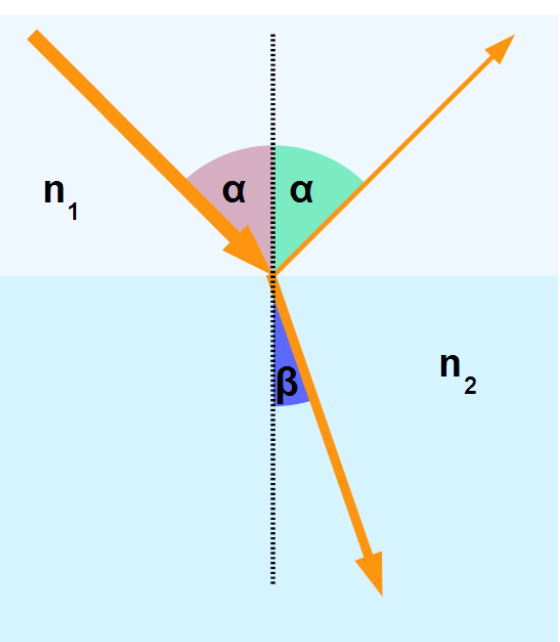
\includegraphics[height=4.75cm]{img/brechung.png} 
						
						\begin{itemize}\itemsep0pt
							\item Wenn ein Lichtstrahl auf die Grenzfläche zwischen zwei Materialien trifft, wird ein Teil des Lichts reflektiert, ein anderer Teil dringt in das Material ein
							\item $\dfrac{sin(\alpha)}{sin(\beta)}=\dfrac{c_{1}}{c_{2}}=\dfrac{n_{2}}{n_{1}}$
							\item $sin(\beta)\leq \dfrac{n_{1}}{n_{2}}$
							\item Der Brechungsindex im Vakuum ist $n_{v} = 1$
						\end{itemize}	
					\end{multicols*}
					
					\subsubsection{Glasfaserkabel}
						\begin{itemize}\itemsep0pt
							\item $\dfrac{c_{G}}{c_{v}}=\dfrac{n_{v}}{n_{G}}$
							\item Lichtgeschwindigkeit Vakuum: $c_{v} = 3\cdot 10^{8}$ m/s 
							\item Signalgeschwindigkeit: $c_{G}$
							\item Brechungsindex Vakuum: $n_{v} = 1$ 
							\item Brechungsindex Glas: $n_{G}$ 
						\end{itemize}	
						
				\section{Thermische Strahlung}
					\begin{itemize}\itemsep0pt
						\item Jedes Objekt mit einer Temperatur grösser 0 K / -273.25 C strahlt elektromagnetische Strahlung ab
						\item Intensität = $\dfrac{\text{Energie}}{\text{Fläche} \times \text{Zeit}}$
						\item Ein Objekt ist in einem thermischen Gleichgewicht, wenn seine Temperatur sich nicht ändert und es ausser Wärmeenergie netto keine Energie aufnimmt oder abgibt
					\end{itemize}
					
					\subsection{Photon}
						\begin{itemize}\itemsep0pt
							\item Energie eines Photons: $E = hv$
							\item $v$: Frequenz
							\item Planck'sche Konstante $h: 6.626\cdot 10^{-34} [Js] $
						\end{itemize}						
					
					\subsection{Absorption Reflexion Emission}
						\begin{itemize}\itemsep0pt
							\item Für einen undurchsichtigen Körper gilt: Alles auftreffende Licht wird geschluckt oder reflektiert
							\item $\alpha$ (Absorptionskoeffizient) wird absoripiert/geschluckt
							\item $\rho = 1 - \alpha$ (Reflexionskoeffizientent) wird reflektiert
							\item Reflexions- und Absorptionskoeffizient können frequenzabhängig sein $\alpha = \alpha(v)$ 
							
							\item $ \alpha_{1\rightarrow 2} + \rho_{1\rightarrow 2} = 1$
							\item Wenn elektromagnetische Strahlung von innen auf die Grenzschicht trifft, kommt es auch zu Reflexion 
							\item Für einen schwarzen Strahler macht es keinen Unterschied, ob ein Strahl von aussen oder innen auf die Trennschicht trifft
							\item Schwarzen Strahler: $ \alpha_{1\rightarrow 2} = \alpha_{2\rightarrow 1} $
							\item Schwarzen Strahler: $ \rho_{1\rightarrow 2} = \rho_{2\rightarrow 1} $
							\item Emission: $ \varepsilon_{2\rightarrow 1} = \alpha_{2\rightarrow 1} $
						\end{itemize}		
						
						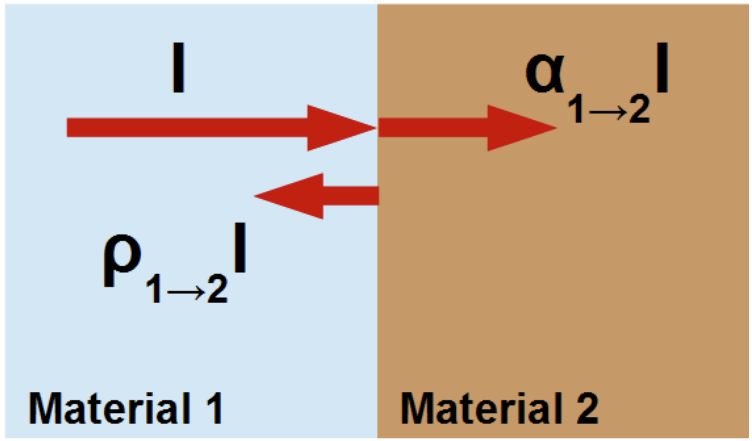
\includegraphics[height=4cm]{img/absopreflex.png} 
					
					\subsection{Schwarzer Körper}
						\begin{itemize}\itemsep0pt
							\item \textbf{Schwarzer Strahler}: für alle Frequenzen $\alpha = 1$ 
							\item Auch ein schwarzer Strahler kann bei hohen Temperaturen leuchten (Sonne)
						\end{itemize}	
						
						\subsubsection{Das Planck’sche Strahlungsgesetz}
							\begin{itemize}\itemsep0pt
								\item Jeder Körper mit einer Temperatur T strahlt einen Mix elektromagnetisches Wellen ab
								\item Für alle schwarzen Strahler ist dieser Mix gleich. Der Mix hängt von der Temperatur aber nicht von der Struktur oder Material ab
								\item $I(v,T)= \dfrac{2h\pi v^{3}}{c^{2}}\dfrac{1}{e^{\frac{hv}{k_{B}T}}-1}$
								\item $I(\lambda ,T)= \dfrac{2h\pi c^{2}}{\lambda^{5}}\dfrac{1}{e^{\frac{hc}{\lambda k_{B}T}}-1}$
								\item Planck'sche Konstante $h: 6.626\cdot 10^{-34} [Js] $
								\item Intensitäten als für verschiedene Temperaturen:
							\end{itemize}	
						
						
							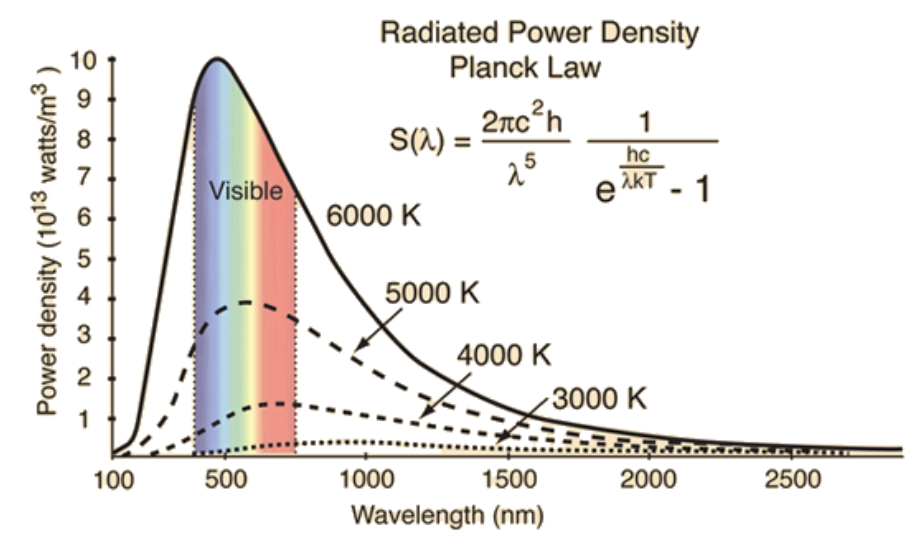
\includegraphics[height=5cm]{img/planck.png} 
							\begin{itemize}\itemsep0pt
								\item Je heisser ein Objekt ist, desto grösser ist die Intensität der thermischen Strahlung
								\item Je heisser ein Objekt ist, desto kürzer ist die Wellenlänge des Hauptteils der Strahlung, bzw. desto höher ist dessen Frequenz

							\end{itemize}	
					
						\subsubsection{Wien’sches Verschiebungsgesetz}
							\begin{itemize}\itemsep0pt
								\item $\lambda_{\text{max}}=\dfrac{b}{T}$
								\item $b = 2.8978 \cdot 10^{-3} [mK]$
								\item Bei hinreichend hoher Temperatur liegt die Wellenlänge $\lambda_{\text{max}}$ im sichtbaren Bereich
								\item Liegt das Strahlungsmaximum im grünen Bereich, gibt es immer rote und blaue Anteile. Unsere Farbwahrnehmung mixt dies zu weisslich
								\item Mit Hilfe des Wien’schen Verschiebungsgesetzes kann die Temperatur eines Sterns bestimmt werden.
							\end{itemize}	
						
						\subsubsection{Stefan - Boltzmann Gesetz}
							\begin{itemize}\itemsep0pt
								\item Gesamtleistung $P_{\text{rad}}$ der Strahlung eines Körpers mit Oberfläche A und Temperatur T
								\item $P_{\text{rad}} = \sigma AT^{4}$
								\item $\sigma = 5.67\cdot 10^{-8} [\dfrac{W}{m^{2}K^{4}}]$
								\item Eine Verdoppelung der Temperatur führt also zu einer Versechzehnfachung der abgestrahlten Leistung
							\end{itemize}	

						\subsubsection{Grauer Körper}
							\begin{itemize}\itemsep0pt
								
								\item Der Emissions-/Absorptionskoeffizient ($\varepsilon/\alpha$) kann von der Temperatur und der Wellenlänge abhängen
								\item Meist spielt die Temperaturabhängigkeit aber keine grosse Rolle
								\item Die Wellenlängenabhängigkeit ist für die meisten Materialien über grosse Wellenlängenbereiche konstant	
							\end{itemize}	
							
						\subsubsection{Energetische Bilanz eines Strahlers}
							\textbf{Thermische Radiation}
							\begin{itemize}\itemsep0pt
								\item $I_{\text{rad,therm}}$ ist die Energiebilanz oder der radiative Energiefluss durch Strahlung
								\item $I_{\text{rad,therm}} = - \dfrac{dE}{dt} = \sigma \varepsilon A(T^{4}-T^{4_{\text{env}}})$
								\item $\varepsilon$: Emissionskoeffizient
							\end{itemize}	
							
							\textbf{Sonneneinstrahlung}
							\begin{itemize}\itemsep0pt
								\item $I_{\text{rad,sun}}$ ist die Energie die von der Sonneneinstrahlung aufgenommen wird
								\item $I_{\text{rad,sun}} = A_{\text{eff}}j_{\text{rad,sol}}= sin(\beta)Aj_{\text{rad,sol}}$
							\end{itemize}
							
							\textbf{Wärmeleitung}
							\begin{itemize}\itemsep0pt
								\item $I_{\text{cond,X,Y}} = -Ah_{\text{X,Y}}(T_{X}-T_{Y})$
							\end{itemize}
							
							\textbf{Energiebilanz}
							\begin{itemize}\itemsep0pt
								\item $I_{\text{rad,sun}}-I_{\text{rad,therm}}-I_{\text{cond}}$
							\end{itemize}	
							
							\textbf{Energiebilanz einer Platte an der Sonne}
							\begin{itemize}\itemsep0pt
								\item $\alpha_{sun}sin(\beta)Aj_{\text{rad,Sol}}-\varepsilon_{IR}A\sigma(T^{4}-T^{4_{\text{Luft}}})-Ah(T^{4}-T^{4_{\text{Luft}}})$
								\item Bei Gleichgewicht ist die Energiebilanz 0
							\end{itemize}
							
						\subsubsection{Skalierungsphänomene}
							\begin{itemize}\itemsep0pt
								\item Verdopplung der Ausmasse eines Systems verdoppelt die Länge, verviertfacht die Oberfläche und verachtfacht das Volumen
								\item Die thermische Bilanz des vergrösserten Systems unterscheidet sich wesentlich von dem ursprünglichen System
								\item Grosse Objekte haben ein Kühlproblem
								\item Nanotechnologie ist Kühlung kaum ein Problem
							\end{itemize}
							
						\subsubsection{Leistung Sonne auf Erde}
						
							\textbf{Albedo}
							\begin{itemize}\itemsep0pt
								\item Intensität der reflektierten Strahlung durch die Intensität der einfallenden Strahlung
							\end{itemize}	
							
							\textbf{Abstrahlung der Sonne}
							\begin{itemize}\itemsep0pt
								\item $P_{\text{sun}} = 4\pi r^{2}_{\text{sun}}\sigma T^{4}_{\text{sun}}$
							\end{itemize}	
							
							\textbf{Intensität der Sonnenstrahlung auf der Erde}
							\begin{itemize}\itemsep0pt
								\item $j_{\text{earth}}= \dfrac{P_{\text{sun}}}{4\pi R_{\text{earth}}^{2}} = \dfrac{r_{\text{sun}}^{2}}{R^{2}_{\text{earth}}}\sigma T^{4}_{\text{sun}}$
							\end{itemize}	
							
							\textbf{Energiebilanz der Erde}
							\begin{itemize}\itemsep0pt
								\item $P_{\text{earth,max}}=j_{\text{earth}}\pi r_{\text{earth}}^{2} = \pi \dfrac{r_{\text{sun}}^{2} r_{\text{earth}}^{2} }{R^{2}_{\text{earth}}}\sigma T^{4}_{\text{sun}}$
								\item $P_{\text{earth,in}}=(1-\text{Albedo})P_{\text{earth,max}}$
								\item $P_{\text{earth,out}}=4\pi r^{2}_{\text{earth}}\sigma T^{4}_{\text{earth}}$
							\end{itemize}	
							
					\section{Fouriertransformation}
						\subsection{Signale}
							\begin{itemize}\itemsep0pt
								\item Signale dienen der Informationsübertragung
								\item Ein Signal ist eine sich räumlich ausbreitende Auslenkung aus einem Grundzustand
								\item Signale werden oft durch Leitmedien übertragen
								\item Die Reaktion des Systems kann gemessen werden
							\end{itemize}
							
							\subsubsection{Amplitude, Periode, Phasenverschiebung}
								\begin{itemize}\itemsep0pt
									\item Die Amplitude A ist das Ausmass der maximalen Auslenkung
									\item Die Periode T gibt die Zeitdauer zwischen zwei Wiederholungen an
									\item Die Frequent v = $\dfrac{1}{T}$
									\item Die verschiebung zischen zwei Signale der selben Form nennt man \textbf{Phasenverschiebung}
								\end{itemize}	
							
							\subsubsection{Sinus Cosinus}
								\begin{itemize}\itemsep0pt
									\item $sin(a-\dfrac{\pi}{2}) = cos(a)$
									\item $cos(a+\dfrac{\pi}{2}) = sin(a)$
								\end{itemize}
							
							\subsubsection{Modulation}
								\begin{itemize}\itemsep0pt
									\item Informationsvermittlung geschieht häufig durch Modulation eines Grundsignals
									\item Sägezahn- und Rechtecksingnale haben theoretisch unendlich steile Flanken
									\item Reale Signale haben immer eine endliche Flankensteilheit
								\end{itemize}	
								
						\subsection{Wellengleichung}
							\begin{itemize}\itemsep0pt
								\item $\dfrac{\partial^{2}f}{\partial t^{2}} = v^{2} \dfrac{\partial^{2}f}{\partial x^{2}} $
								\item $v=\dfrac{\omega}{k}$
								\item Alle Funktionen einer bestimmten Form, somit auch eine bestimmte Form von Sinus- und Cosinusfunktionen, sowie deren Summen sind Lösungen der Wellengleichung
								
								\item Jede Funktion kann als Summe von Sinus – und Cosinusfunktion dargestellt werden (Fouriertransformation)
								\item Die Summe von Lösungen der Wellengleichung ist auch eine Lösung der Wellengleichung
								\item Jedes Audiosignal kann also als Summe von reinen Tönen dargestellt werden
								\item Jedes sichtbare elektromagnetische Signal kann als Summe von Regenbogenfarben dargestellt werden
							\end{itemize}	
							
						\subsection{Fourierzerlegung}
							\begin{itemize}\itemsep0pt
								\item $f(t)=\dfrac{a_{0}}{2}+\sum_{k=1}^{\infty}(a_{k}cos(2\pi v_{k}t)+b_{k}sin(2\pi v_{k}t))$
								\item $a_{k}, b_{k}$: Fourierkoeffizienten
								\item $a_{k} = \dfrac{2}{T} \int_{-\dfrac{T}{2}}^{\dfrac{T}{2}}f(t)cos(2\pi v_{k}t)\delta t$
								\item $b_{k} = \dfrac{2}{T} \int_{-\dfrac{T}{2}}^{\dfrac{T}{2}}f(t)sin(2\pi v_{k}t)\delta t$
								\item $v_{k} = \dfrac{k}{T}$
							\end{itemize}	
							
							\subsubsection{Komplexe Darstellung}
								\begin{itemize}\itemsep0pt
									\item $f(t)= \sum_{k=-\infty}^{\infty} c_{k} \cdot e^{2\pi i v_{k}t}$
									\item $c_{k} = \dfrac{1}{T} \int_{0}^{T}f(t) e^{-2\pi i v_{k}t} \delta t$
								\end{itemize}
								
							\subsubsection{Amplituden- und Phasendarstellung}
								\begin{itemize}\itemsep0pt
									\item $U(t) = f(t)=\dfrac{a_{0}}{2}+\sum_{k=1}^{\infty} A_{k} cos(2\pi v_{k}t - \varphi_{k})$
									\item $A_{k}=\sqrt{a_{k}^{2} + b_{k}^{2}}$
									\item $\varphi_{k} = arccos(\dfrac{a_{k}}{A_{k}}) =arcsin(\dfrac{b_{k}}{A_{k}}) $
								\end{itemize}	
								
								
							\subsubsection{Spektrum/ Frequency Domain Representation}
								\begin{itemize}\itemsep0pt
									\item Die Amplituden $A_{k}$ als Funktion von k nennt man Spektrum oder frequency domain representation von U(t)
									\item Die Phasen $\varphi_{k}$ als Funktion von k nennt man das Phasendiagramm von U(t)
								\end{itemize}	
								
								
						\subsection{Töne und Klangfarben}		
							\begin{itemize}\itemsep0pt
								\item Musikinstrumente produzieren mehrere Schwingungen gleichzeitig
								\item Neben dem Grundton erzeugt jedes Instrument auch Obertöne
								\item Die Mischung der Obertöne bilden den typischen Klang eines Instruments.
								\item Je mehr Obertöne ein Audiosignal enthält, desto schärfer tönt ein Instrument.
							\end{itemize}	
						
						\subsection{Reale Signale}		
							\begin{itemize}\itemsep0pt
								\item Wenn mit Messwerten gearbeitet wird sind diskrete Punkte bekannt
								\item $g(t_{r}) = g_{r} = \dfrac{1}{N} \sum_{s=1}^{N} w_{s} e^{2\pi i f_{s}t_{r}}$
								\item $w_{s}  = \sum_{r=1}^{N} w_{s} e^{-2\pi i f_{s}t_{r}}$
								\item $f_{s} = \dfrac{(s-1)}{T}$
								\item $t_{r} = \dfrac{(r-1)T}{N}$
							\end{itemize}	
							
						\subsection{Nicht Periodische Signale}		
							\begin{itemize}\itemsep0pt
								\item Die Idee der Fouriertransformation basiert auf der Annahme periodischer Funktionen
								\item Die meisten natürlichen Signale sind nicht periodisch
								\item In der Praxis wird ein Abschnitt gemessen und dieser vervielfacht, damit ein periodisches Signal entsteht
								
							\end{itemize}	
							
						\subsection{Nyquist - Shannon Theorem}		
							\begin{itemize}\itemsep0pt
								\item Die Anzahl Messpunkte und die Dauer des Messintervalls bestimmen die tiefste und höchste messbare Frequenz
								\item Um ein Signal, welches aus Fourierkomponenten mit maximaler Frequenz $f_{\text{max}}$ zusammengesetzt ist, voll ständig zu rekonstruieren, muss man eine diskrete Fouriertransformation mit mindestens \textbf{$N >2Tf_{\text{max}}$} Messpunkten durchführen
								\item Um das Spektrum einer Funktion bis zur Frequenz $f_{\text{max}}$ auszumessen, muss mindestens mit doppelter Frequenz gemessen werden
								\item Um das Spektrum einer Funktion bis zur Frequenz $f_{\text{min}}$ auszumessen, muss über ein Zeitintervall $T > \dfrac{1}{f_{\text{min}}}$ gemessen werden
							\end{itemize}	
							
						\subsection{Aliasing}		
							\begin{itemize}\itemsep0pt
								\item Wenn das Nyquist - Shannon Theorem nicht eingehalten wird, entsteht der Aliasing/Alias Effekt
								\item In einer Analyse erscheinen tiefe Schwingungen, welche im Originalsignal als hohe Schwingungen vorhanden sind
								\item Mit mathematischen und messtechnischen Methoden können hohe Frequenzen unterdrückt werden
							\end{itemize}	
						
						\subsection{Unschärfe, Blip und Knall}		
							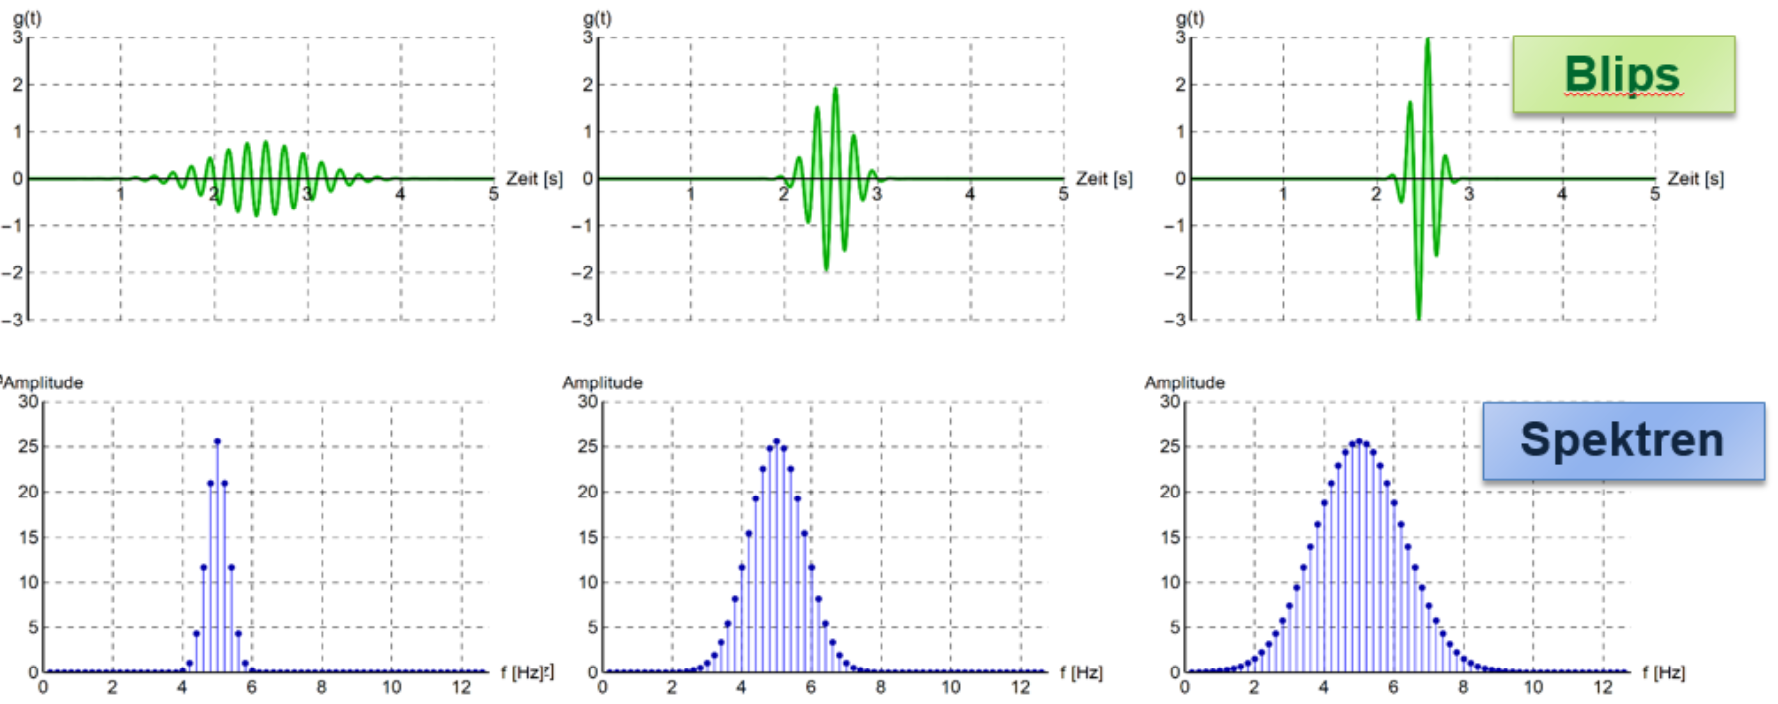
\includegraphics[height=3.5cm]{img/blip.png} 
							\begin{itemize}\itemsep0pt
								\item Ein Blip besteht aus vielen Frequenzen, lokalisiert um die "Hauptfrequenz" $v_{0}$
								\item Je schmaler das Blip, desto breiter das Spektrum
							\end{itemize}	
							
							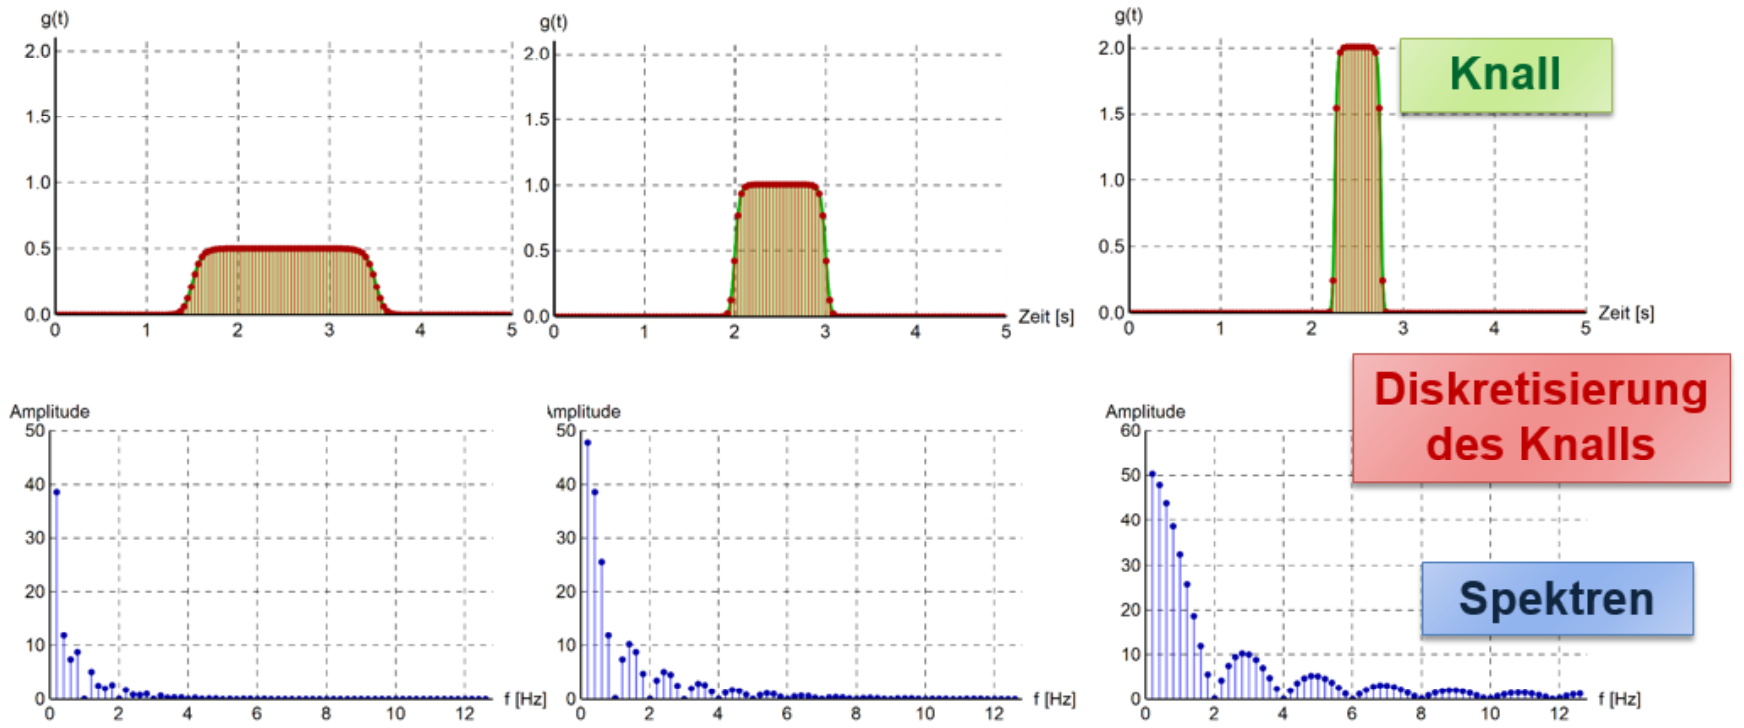
\includegraphics[height=3.75cm]{img/knall.png} 
							\begin{itemize}\itemsep0pt
								\item Ein Knall ist eine kurze starke Auslenkung eines Systems
								\item Je kürzer und stärker der Knall, desto breiter ist das Spektrum
							\end{itemize}	
							
							\textbf{Unschärfe}
							\begin{itemize}\itemsep0pt
								\item Je lokalisierter ein Signal in der Zeitdomäne ist, desto mehr Frequenzen sind zu seiner Darstellung nötig
								\item Je lokalisierter ein Signal in der Zeitdomäne ist, desto delokalisierter ist es im Frequenzraum
								\item Die Aussage gilt für jede Art von Signal
								\item Je steiler die Flanken eines Signals, desto grösser der Anteil der hohen Frequenzen im Signal
							\end{itemize}	
							
							\textbf{Unschärferelation}
							\begin{itemize}\itemsep0pt
								\item $\dfrac{\Delta f\cdot \Delta t}{2} \approx 1$
							\end{itemize}	
							
							\textbf{Musik}
							\begin{itemize}\itemsep0pt
								\item Damit man einen Ton als harmonisch empfindet, muss eine Frequenz dominieren
								\item Damit die Frequenz der Grundschwingung dominiert, muss das Signal lange genug sein
								\item Das Ohr ist aber wie die meisten Messinstrumente ein relatives Organ
								\item Den Unterschied zwischen 380 und 400 Hz kann man hören, den zwischen 9980 und 10000 Hz nicht
								\item Instrumente mit tiefen Frequenzen müssen lange Töne produzieren, um gut zu tönen
								\item Bei hohen Tönen werden grössere Frequenzunschärfen als harmonisch empfunden
							\end{itemize}	
							
						\subsection{Messdauer und Trennschärfe}		
							\begin{itemize}\itemsep0pt
								\item Bei einer Signallänge T und N = 2n Messpunkten ergeben sich Amplituden für die Frequenzen $f_{s}$
								\item $f_{s}=0,\dfrac{1}{T},\dfrac{2}{T},...,\dfrac{n-1}{T},\dfrac{n}{T}$
								\item Je länger das Signal, desto kleiner ist die Differenz zwischen den Frequenzen
								\item Je länger das Signal, desto kleiner ist die Maximalfrequenz in der Fourierreihe
								\item Je mehr Messpunkte, desto höhere Frequenzen können erfasst werden
							\end{itemize}	
							
						\subsection{Absorption von LIcht}		
							\begin{itemize}\itemsep0pt
								\item Ein Lichtstrom mit Intensität $I_{L}$ besteht aus Photonen
								\item Trifft Licht auf einen Absorber, wird ein Teil des Lichts reflektiert, der Rest tritt in den Absorber ein
								\item Im Absorber hat ein Photon pro zurückgelegte Wegstrecke eine Wahrscheinlichkeit $\dfrac{1}{\lambda}$ , absorbiert zu werden
							\end{itemize}	
							
							\textbf{Abschwächung der Intensität}
							\begin{itemize}\itemsep0pt
								\item $I_{L}(x)=I_{L,0}e^{-\dfrac{x}{\lambda}}$ 
								\item $I_{L,0}$: Intensität bei x = 0
							\end{itemize}	
						
						\subsection{Dispersion}		
							\begin{itemize}\itemsep0pt
								\item Dispersion bezeichnet das Phänomen, dass die Phasengeschwindigkeit einer Welle von der Frequenz abhängt
								\item Elektromagnetische Wellen die sich in Materie ausbreiten, zeigen Dispersion.
							\end{itemize}	

						\subsection{Resonanz}		
							\begin{itemize}\itemsep0pt
								\item Systeme können durch äussere Anregungen in Schwingung versetzt werden
								\item Die Anregungen können Schwingungen sein
								\item Bestimmte Frequenzen führen zu grossen Schwingungen, andere Frequenzen haben praktisch keine Wirkung
								\item Frequenzen die zu grossen Schwingungen führen sind Resonanzfrequenzen
								\item Je geringer die Reibung, desto grösser die Resonanzamplitude
								
							\end{itemize}	
						\subsection{Lärm}	
							\subsubsection{Intensität}	
								\begin{itemize}\itemsep0pt
									\item Tritt eine Welle mit einer Intensität I auf eine Fläche A ist die Leistung P:
									\item $P=I\cdot A$
									\item $I = 2\pi^{2}\rho_{0}f^{2}s_{\text{max}}^{2}v = \dfrac{1}{2}\dfrac{p_{\text{max}}^{2}}{\rho_{0}v}$ (harmonische Schallwelle)
									\item $\rho_{0} = 1.2 kg/m^{3}$
									\item $s_{\text{max}}$: Maximale Auslenkung der Luftmoleküle aus der Ruhelage
									\item $p_{\text{max}}$: Der maximale auftretende Schalldruck
									\item $v$: Schallgeschwindigkeit
									\item $I=\dfrac{P}{4\pi R^{2}}$ (Intensität bei Abstand R der Quelle)
								\end{itemize}	
							
							\subsubsection{Dezibel}
								\begin{itemize}\itemsep0pt
									\item Der Unterschied zweier Intensitäten in Dezibel ist Q
									\item $Q = 10 \cdot log_{10}(\dfrac{I_{1}}{I_{2}}) dB$
									\item Das Schallempfinden ist nicht proportional zur Schallintensität
									\item Der \textbf{Schallintensitätspegel H} ist proportional zum Logarithmus der Schallintensität I
									\item $H = (10dB) \cdot log_{10}(\dfrac{I}{I_{0}})$
									\item $I_{0} = 10^{-12}\dfrac{W}{m^{2}}$
								\end{itemize}	
								
							\subsubsection{Information}
								\begin{itemize}\itemsep0pt
									\item Im technischen Kontext hat Lärm weniger mit Lautstärke sondern mehr mit Informationsgehalt zu tun
								\end{itemize}	
								
								\textbf{iid-Lärm}
								\begin{itemize}\itemsep0pt
									\item $\Lambda(t)$
									\item identically and independently distributed
									\item Das Signal $\Lambda(t)$ ist eine Zufallsvariable
									\item Die Wahrscheinlichkeitsverteilung ist für alle Zeitpunkte gleich
									\item Der Zufallswert zu einem Zeitpunkt $\Lambda(t_{1})$ ist unabhängig vom Zufallswert an einem anderen Zeitpunkt $\Lambda(t_{2})$
									\item Bei recht beträchtlichen Lärmniveaus kann das Signal immer noch erkannt werden. Für hohe Lärmniveaus ist das aber schwierig
								\end{itemize}	
								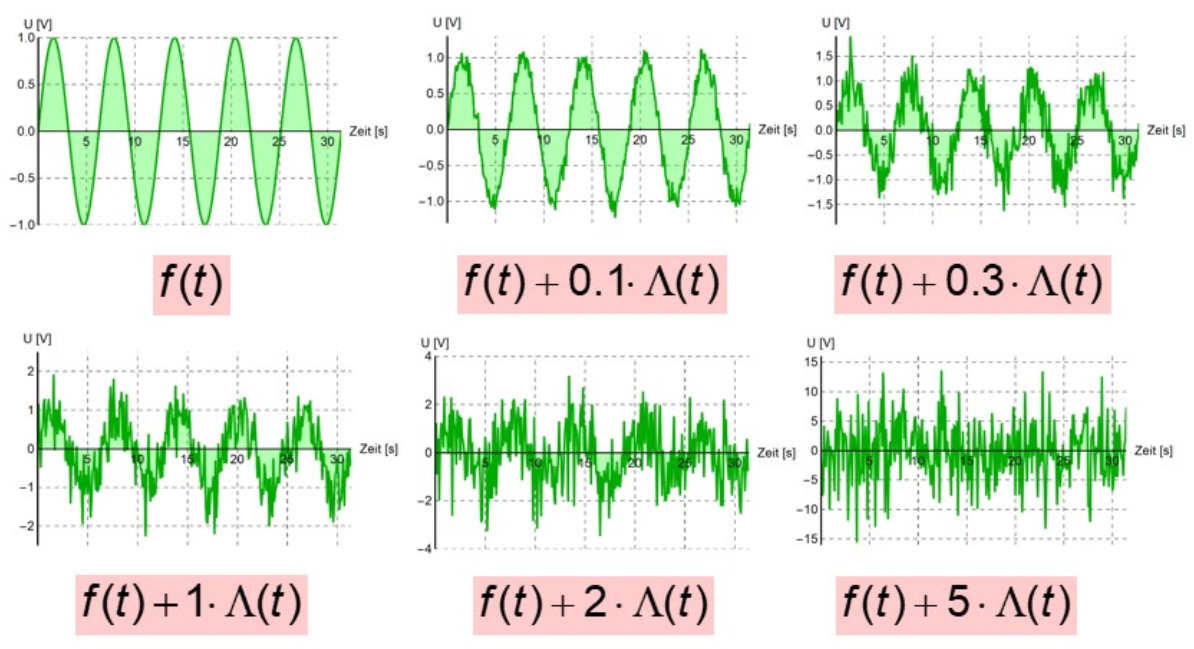
\includegraphics[height=4.75cm]{img/laerm.png} 
								
							\subsubsection{Thermisches Rauschen}
								\begin{itemize}\itemsep0pt
									\item In einem Widerstand R besteht eine fluktuierende Spannung mit Mittelwert $U_{\text{term,eff}}$
									\item $U_{\text{term,eff}} \approx \sqrt{TR}$
									\item Rauschen ist proportional zur Wurzel der Temperatur und dem Widerstand
								\end{itemize}	
								
							\subsubsection{Singal-to-Noise Ratio}
							\begin{itemize}\itemsep0pt
									\item SNR $=\dfrac{P_{\text{signal}}}{P_{\text{noise}}}=\dfrac{I_{\text{signal}}}{I_{\text{noise}}}$
									\item SNR $=\dfrac{A_{\text{signal}}^{2}}{A_{\text{noise}}^{2}}$
									\item Die Leistung/Intensität eines Signals ist in der Regel proportional zum Quadrat der Amplituden
								\end{itemize}	
								


\end{multicols*}

% Dokumentende
% ======================================================================
\end{document}
